\chapter{Detector Characterization}
\label{chap:DetChar}
Repeated characterization techniques of the detector materials are necessary to ensure a fair comparison between different detector materials.
As the focus of this work was on effective scintillators the characterizations were designed to measure scintillation properties; namely the light yield of the detector and the count rate when exposed to different radiation sources.

\begin{itemize}
  \item Total Neutron Counts – provides a measure of how responsive the detector is to neutrons
  \item  Total Neutron Count Rate Per mg Absorber – provides a measure of how well the fabricated detector utilizes the neutron absorber in it. Indirectly this can be a measure of the amount of absorber in the detector
  \item  Gamma LLD – The position (in channel number) of where an LLD would have to be set in order to meet the criteria of \si{1E-6}
  \item  Fraction of Total Neutron Count Rate Above the Gamma LLD – this is a measure of how effective the film would be with an LLD set in order to meet the This is calculated by summing the counts above the gamma LLD and dividing by the total counts.
  \item  Alpha Peak – provides a clear indication of the light yield of the film from an alpha particle, which is one of the reaction products of the 6Li neutron interaction. The alpha peak is visible in thin films when other features may be lost (due to the range of the secondary electrons exceeding the thickness of the detector) because the range of the alpha is on the order of 30 microns.
  \item  Beta Average – characterizes the response of the film to electrons, account for the possibility that a film may not have a clearly defined feature due to energy escaping. Electrons are generated in the film from scattering events of photon interactions.
  \item  Alpha / Beta – characterizes the relative light yield of the detector from heavy charged particles to electrons.
  \item  Pulse Height Deficit – a measure the apparent energy loss (as seen from the pulse height) of a heavy charged ion compared to an electron. This is measured as the difference between the energy of the heavy ion and its apparent energy from the pulse height. It should be noted that this term closely resembles the phenomena described by pulse height defect as seen in semiconductors.
  \item  Photons per Neutron – a measure of the light yield of the film, or how many photons are produced per energy absorbed.
\end{itemize}

\subsection{Characterization Electronics and Sources}
Solid samples are characterized by mounting them with a thin layer of silicone optical grease (BC-630, index of refraction 2.465) onto a Philips XP2202B 10 Stage PMT most sensitive in the \SI{350}{\nm} to \SI{500}{\nm} region.
The PMT is then connected to a Canberra 2007P base, which also functions as a preamplifier.
The Canberra 2007P feeds into an Ortec 572A amplifier, and the amplified signal is inputted to an Ortec 926 MCB-ADC.
MAESTRO-32 is the used to read the signals from the MCB.
\autoref{fig:ElectronicsSetup} provides an overview of this setup.
\begin{figure}
  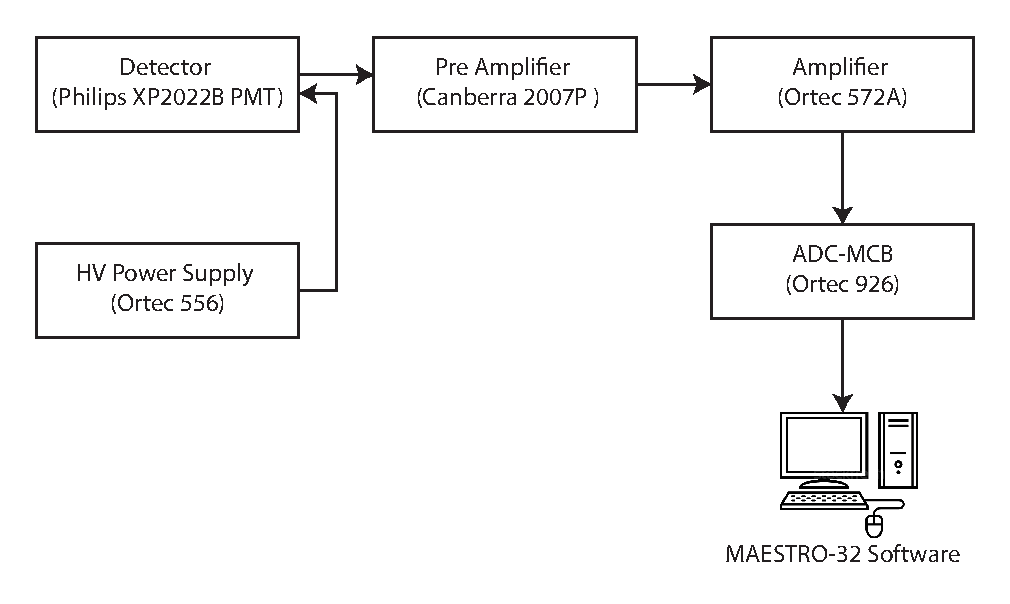
\includegraphics[width=0.5\textwidth]{ElectronicsSpectra}
  \caption[Optical Characterization Experiment Setup]{Electronic figure for measuring the spectra of materials in response to various radiation sources.}
  \label{fig:ElectronicSetup}
\end{figure}
A general protocol has been developed in order to ensure that the measurements are made in a repeatable manner and verified with a reference.
\begin{enumerate}
  \item Verify that the instrumentation gains are stable by confirming that the reference neutron peak is in the same channel as for previous measurements. This is completed by setting the voltage and coarse gain to previously determined values, and then adjusting the fine gain until the peak of the lead spectra measurement occurs in the specified location,
  \item obtain a spectrum from an Am-241 alpha source,
  \item obtain a spectrum from a Cl-36 beta source,
  \item obtain a neutron spectrum from the Pb-shielded tube neutron irradiator,
  \item obtain a neutron spectrum from the Cd-shielded tube in the neutron irradiator,
  \item obtain a gamma spectrum in the gamma irradiator.
\end{enumerate}

\subsubsection{Neutron and Gamma Irridiators}
The neutron irradiator is a custom built \SI{0.59}{\ug} \iso[252]{Cf} source encased in 2” blocks of high density polyethylene (HDPE). 
The HDPE box is approximately 20” long, 12” wide, and 14” tall (\autoref{fig:NeutronIrridiator}). 
There are two detector 1/16” thick acrylic detectors wells, one surrounded by a 1/16” cadmium to shield out thermal neutrons, and the other surrounded by 1/16” of lead to shield out a similar amount of gammas as the cadmium well.
The \iso[252]{Cf} source is surrounded by stainless steel, which in turn is contained within a 2” diameter, 1/2” thick, 5 and 1/4” tall lead vessel.
\begin{figure}
  \centering
  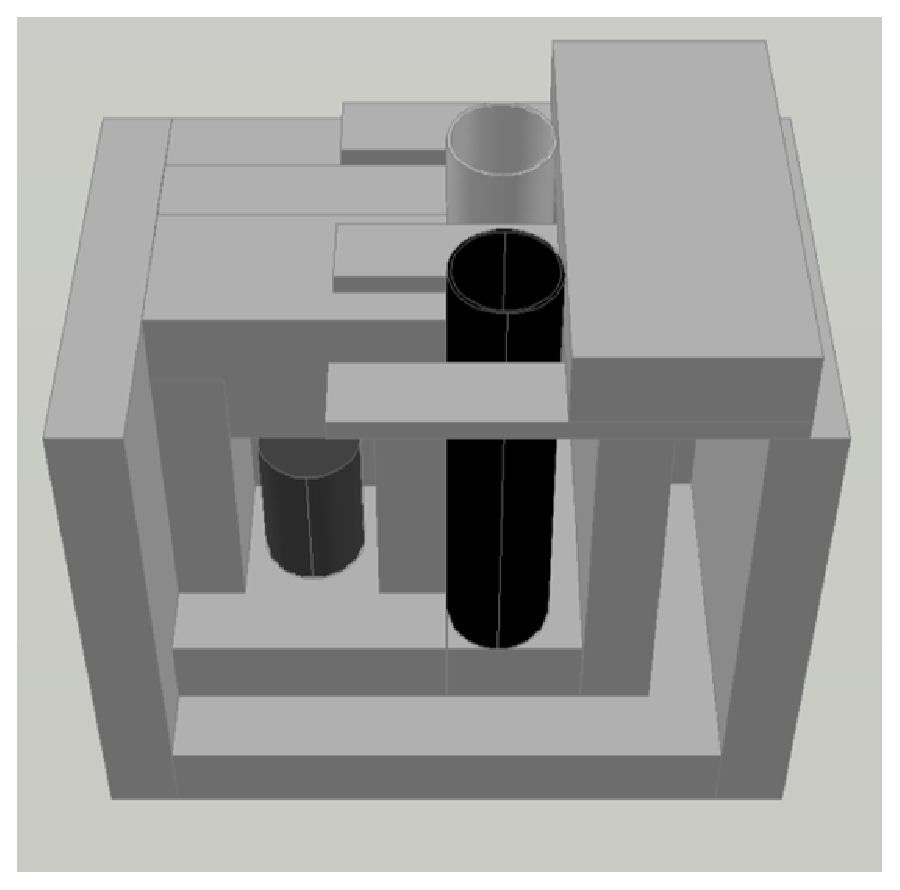
\includegraphics[width=0.5\textwidth]{NeutronIrridiator_CAD}
  \caption[CAD Rendering of Neutron Irridiator]{Schematic of the neturon irridiator.}
  \label{fig:NeutronIrridiator}
\end{figure}
The gamma sources consist of button sources (\iso[137]{Cs} up to \SI{10}{\u Ci} and \iso[60]{CO} up to \SI{1}{\u Ci}) as well as a gamma irradiator that produces a 10 mR/hr gamma field across the detector face. 
The irradiator consist of four 4”x8”x 2” lead bricks on the bottom with and additional four 4”x4”x2” lead bricks encased in an 1/8” metal box. 
The top four inches is HDPE. 
The overall dimensions of the detector are 14” by 12” by 12”. 

\section{Light Yeild}
The light yield of a spectrum describes how many photons are generated (and subsequently detected on a PMT) for a given material for a scintillation event from a radiation source.
In general, a feature, such as the Compton edge or neutron peak,  provides a unambiguous measure of light yield of a film. 
However, the thinner films do not always have such a clearly defined feature, and thus an alternative measure needs to be formulated.
The spectral average is then defined as \eqref{eqn:spectralAverage} where \definevar{p(x)}{measured spectrum} and \definevar{x} {channel number} which describes the count rate average channel number, normalized by the total count rate.
\begin{align}
	<\mu> = \frac{\int_0^\infty x p(x) dx}{\int_0^\infty p(x) dx}
	\label{eqn:spectralAverage}
\end{align}
The limits of integration in \eqref{eqn:spectralAverage} are from the lowest to the highest channel number.
While the spectral average does provide a clear representation of a spectra, it fails to capture the shape of the spectra and tends to underestimate the spectra, as most spectra a skewed having the majority of their counts in the low channel region.

The light yield of fabricated samples that were characterized was completed by comparing the spectrum average of a sample to that a sample of a known light yield.
This is shown for neutrons in \eqref{eqn:neutronLY}, and for gammas in \eqref{eqn:gammaLY}.
GS20 is normally used as the reference sample, having a reported light yield of \SI{3,800}{photons \per\MeV} and \SI{6,200}{photons \per neutron} \cite{carel_w.e_inorganic-scintillator_2001,knoll_radiation_2009}.
\begin{align}
	LY_{n,\text{sample}} &= LY_{n,\text{ref}} \left( \frac{<n>_\text{sample}}{<n>_\text{ref} } \right )\\
	&= \SI{6,200}{photons\per neutron} \left( \frac{<n>_\text{sample}}{<n>_\text{ref} } \right )
	\label{eqn:neutronLY}
\end{align}
\begin{align}
	LY_{\gamma,\text{sample}} &= LY_{\gamma,\text{ref}} \left( \frac{<\gamma>_\text{sample}}{<\gamma>_\text{ref} } \right )\\
	&= \SI{3,800}{photons\per\MeV} \left( \frac{<\gamma>_\text{sample}}{<\gamma>_\text{ref} } \right )
	\label{eqn:gammaLY}
\end{align}

\section{Intrisinic Efficiency}
\label{sec:IntEff}

Often times it is necessary to relate the performance of a detector to number of particles that cross the detector, this is completed using the intrinsic efficiency.
Thus the intrinsic efficiency it is a measure at how efficient the detector is at detecting radiation, normalized to the amount of radiation that crosses the detector.
The intrinsic efficiency is defined as the ratio between the counts recorded in the detector and the number of impingement radiation on the detector\cite{knoll_radiation_2009}, expressed as \eqref{eqn:intEffDef},
\begin{align}
  \label{eqn:intEffDef}
  \epsilon_{int} = \frac{N_c}{N_i}
\end{align}
where:
\begin{itemize}
  \item[] \definevar{$\epsilon_{int}$}{intrinsic efficiency},
  \item[] \definevar{$N_c$}{number of counts recorded by the detector}, and
  \item[] \definevar{$N_i$}{quanta of radiation incident upon the detector}.
\end{itemize}
In order to determine the intrinsic efficiency of a detector it is then necessary to determine the performance of the detector (easily completed by measuring the detector) and the number of radiation impingement upon the detector (usually accomplished through calculation on simulation).

The quanta of radiation incident upon the detector can be expressed as the product of two components: the source strength and the solid angle, \eqref{eqn:QuantaIncidentDef},
\begin{align}
  \label{eqn:QuantaIncidentDef}
  N_i = \Omega S_0
\end{align}
where:
\begin{itemize}
  \item[] \definevar{$S$}{source strength}, and 
  \item[] \definevar{$\Omega$}{fraction of solid angle detector subtends}.
\end{itemize}
Radiation sources generally decay from their initial source strength according to the half-life of the source.
The time dependent source strength, $S(t)$ can then be expressed as \eqref{eqn:HalfLife}, where \definevar{$S_0$}{initial source strength}, \definevar{$t_{1/2}$}{half life} and \definevar{$t$}{age of source}.
\begin{align}
  \label{eqn:HalfLife}
  S(t) = S_0 e^{-\frac{\ln{2}}{t_{1/2}} t}
\end{align}

The fraction of the source solid angle the detector subtends, $\Omega$, is computed using MCNPX. 
A F1 tally, defined in \eqref{eqn:F1Def}, is employed over the detector surface with two cosine bins, $-1<\cos\theta<0$ and $0<\cos\theta<1$, which divide the tally into particles that enter the surface and particles that leave the surface, respectively.
\begin{align}
  \label{eqn:F1Def}
  F1 &= \int_A dA \int_E dE \int_{4\pi} d\Omega ;;\vec{n}\cdot\vec{J}(\vec{r},E,\vec{\Omega}) \\
 %  &= \int_A dA \int_E dE \int_{4\pi} d\Omega \vec{n}\cdot\vec{\Omega}\Phi(\vec{r},E,\vec{\Omega}) \notag
\end{align}
In \eqref{eqn:F1Def} the position $\vec{r}$\nom{$\vec{r}$}{position}, direction $\vec{\Omega}$\nom{$\vec{\Omega}$}{direction} and energy $E$ \nom{$E$}{energy} dependent particle current $\vec{J}$ \nom{$\vec{J}$}{particle current} is integrated over the entire area, energy and direction normal to the surface of the area.
As macro-bodies are used for the surfaces of the detector, $-1<\cos\theta<0$ represents the particles that cross into the surface and $0<\cos\theta<1$ the particles that leave the surface.
In the case where macrobodies are not used to create the cell, the reader is referred to the MCNPX manual for more details.

The count rate of a detector is found by integrating the measured spectra, $p(x)$, \nom{$p(x)$}{measured spectra as a function of channel number $x$} over some bounds of integration.
It is then possible to express the intrinsic efficiency as a function of a mathematical lower level discriminator (MLLD) of the measured spectra \footnote{The MLLD behaves essentially as a physical lower level discriminator in that all counts below this value are discarded.} in order to determine at what MLLD the intrinsic efficiency is less then a value.
Equation \eqref{eqn:MLLDDef} shows such a formulation of the intrinsic efficiency as a function of a MLLD, where the upper bond is assumed to be the end of the spectra or highest recorded channel of the analog to digital converter.
\begin{align}
	\label{eqn:MLLDDef}
	\epsilon_{int}(MLLD) &= \frac{\int_{MLLD}^\infty p(x)dx}{N_i}
\end{align}

\subsection{Neutron Intrinsic Efficiency}
The number of counts upon a detector is measured by irradiating the detector in a lead and cadmium well of the neutron irridiator to determine $N_i$, and then simulating that geometry in bench-marked MCNPX in order to determine the number of neutrons incident on the detector\footnote{MCNPX simulations were benched-marked against GS20 and against polymer films, having 4\% and 15\% agreement to measured count rate, respectively.}.
The determination of $N_i$ consists of two parts: 1) determining the number of neutrons crossing the detector surface in the lead and cadmium wells and, 2) determining the source strength.
The \iso[252]{Cf} source was \SI{0.59}{\ug} on July 2, 2009.
Given that the half-life of \iso[252]{Cf} is 2.64 years and \iso[252]{Cf} has a spontaneous neutron emission rate of \SI{2.3E6}{neutron\per\second\per\micro\gram} the time dependent source strength can be calculated as \eqref{eqn:Cf252SourceStrength}.
\begin{align}
  \label{eqn:Cf252SourceStrength}
  S(t) &= S_0 e^{-\frac{\ln{2}}{t_{1/2}} t} \\ \notag 
    &= \SI{0.59}{\ug} \iso[252]{Cf} \;\frac{\SI{2.3E6}{neutron\per\second}}{\si{\ug} \iso[252]{Cf}}\; e^{-\frac{ \ln{2}}{\SI{2.64}{year}}t}  \\ \notag
    &= \SI{1.357E6}{neutron\per\second}\; e^{-\frac{ \ln{2}}{\SI{2.64}{year}}t} 
\end{align}

Table \ref{tab:NeutronSolidAngle} summarizes the incident flux for a number of different detector sizes and heights.
The fraction of solid angle subtended by other geometries can be computed by interpolation on the values of this table, as shown in the examples calculations.
It should be noted that there is considerable variation in the neutron flux in the detector wells, as shown in Figure \ref{fig:NeutronFluxProfiles}.
Thus, even though the calculations are accurate to less than a percent, the physical error on the intrinsic efficiency will be much higher due to uncertainty in where the detector was placed in the well.

\begin{table}
	\centering
	\caption[Simulated Thermal Neutron Solid Angle for Various Film Radii]{Simulated Neutron Solid Angle for Various Film Radii in the net spectra. The film radii are shown in seperate columns, with the thickness in rows. The thermal spectra (shown) is the subtraction of the lead and cadmium wells.}
	\label{tab:NeutronSolidAngle}
	\begin{tabular}{c | c c c c c c}
Thickness (\si{\cm})	&	\SI{1}{\cm}	&	\SI{1.27}{\cm}	&	\SI{1.905}{\cm}	&	\SI{2}{\cm}	&	\SI{2.5}{\cm}	&	\SI{2.54}{\cm} \\ \hline
0.0025	&	0.00055	&	0.00089	&	0.00204	&	0.00225	&	0.00351	&	0.00362	\\
0.005	&	0.00055	&	0.00090	&	0.00204	&	0.00224	&	0.00350	&	0.00361	\\
0.01	&	0.00055	&	0.00089	&	0.00204	&	0.00223	&	0.00348	&	0.00359	\\
0.015	&	0.00055	&	0.00089	&	0.00202	&	0.00222	&	0.00346	&	0.00357	\\
0.03	&	0.00056	&	0.00090	&	0.00201	&	0.00221	&	0.00341	&	0.00353	\\
0.1	&	0.00058	&	0.00093	&	0.00202	&	0.00220	&	0.00334	&	0.00347	\\
0.2	&	0.00063	&	0.00099	&	0.00208	&	0.00225	&	0.00338	&	0.00349	\\
0.5	&	0.00080	&	0.00119	&	0.00234	&	0.00251	&	0.00365	&	0.00375	\\
1	&	0.00109	&	0.00159	&	0.00286	&	0.00306	&	0.00427	&	0.00437	\\
2	&	0.00170	&	0.00233	&	0.00389	&	0.00412	&	0.00544	&	0.00555	\\
	\end{tabular}
\end{table}
\begin{figure}
	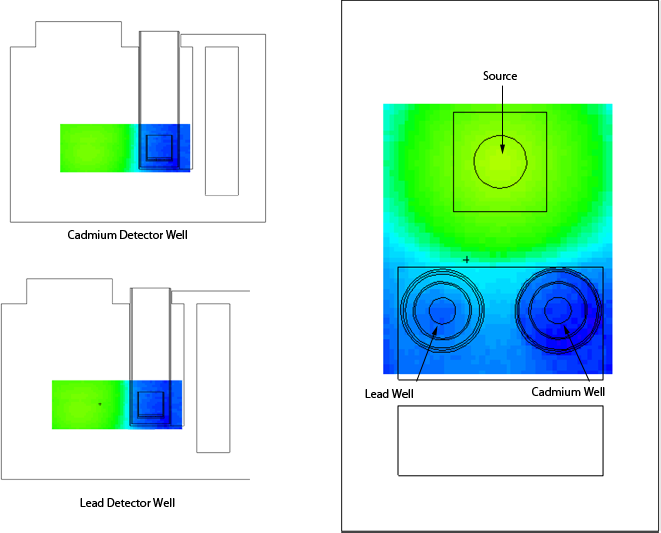
\includegraphics[width=\textwidth]{SpatialNeutronFlux}
  \caption[Neutron Flux Profiles of the Lead and Cadmium Wells]{Neutron Flux Profiles of the Lead and Cadmium Wells. Lighter colors correspond to a higher neutron population. The effect of the cadmium shielding is observed in the depression of the flux in the lower right by the cadmium well.}
  \label{fig:NeutronFluxProfiles}
\end{figure}

\subsection{Gamma Intrinsic Efficiency}
The gamma irridiator consists of a \SI{97}{\micro Ci} \iso[60]{Co} (January 1st, 2012) inside of a steel pipe encased in lead bricks.
The gamma intrinsic efficiency is calculated by simulating the fraction of solid angle the detector subtends and then using radioactive decay to model the \iso[60]{Co} source.
The \iso[60]{Co} source strength is calculated according to \eqref{eqn:Co60SourceStrength}. 
As there are two photons emitted from each \iso[60]{60} decay, in order to normalize the MCNPX source strength it is necessary to multiply the single photon activity by two.
Tabulated solid angle fractions are in Table \ref{tab:GammaSolidAngle}, and once again interpolation can be used for geometries not enumerated.
These values were extracted from an MCNPX simulation using an F1 tally as described above.
\begin{align}
  \label{eqn:Co60SourceStrength}
  S &= S_0 e^{-\frac{\ln{2}}{t_{1/2}} t} \\ \notag 
    &= \SI{97}{\micro Ci} \iso[60]{Co}\; \frac{\SI{3.7E10}{decay\per\second}}{\si{Ci}} \;\frac{2\text{photon}}{decay}\;e^{-\frac{ \ln{2}}{\SI{5.27}{year}}t}  \\ \notag
    &= \SI{7.178E6}{photon\per\second}\;e^{-\frac{ \ln{2}}{\SI{5.27}{year}}t} 
\end{align}
\begin{table}
	\centering
	\caption{Simulated Gamma Solid Angle for Various Film Radii}
	\label{tab:GammaSolidAngle}
	\begin{tabular}{c | c c c c c c}
Thickness (\si{\cm})	&	\SI{1}{\cm}	&	\SI{1.27}{\cm}	&	\SI{1.905}{\cm}	&	\SI{2}{\cm}	&	\SI{2.5}{\cm}	&	\SI{2.54}{\cm} \\ \hline
0.0025	&	0.0060	&	0.0095	&	0.0206	&	0.0226	&	0.0347	&	0.0357\\
0.005	&	0.0060	&	0.0095	&	0.0206	&	0.0226	&	0.0347	&	0.0357\\
0.01	&	0.0060	&	0.0095	&	0.0206	&	0.0226	&	0.0347	&	0.0357\\
0.015	&	0.0060	&	0.0095	&	0.0206	&	0.0226	&	0.0347	&	0.0357\\
0.03	&	0.0060	&	0.0095	&	0.0206	&	0.0227	&	0.0347	&	0.0357\\
0.1	&	0.0060	&	0.0096	&	0.0207	&	0.0227	&	0.0348	&	0.0358\\
0.2	&	0.0061	&	0.0097	&	0.0209	&	0.0229	&	0.0349	&	0.0360\\
0.5	&	0.0063	&	0.0099	&	0.0212	&	0.0232	&	0.0353	&	0.0364\\
1	&	0.0066	&	0.0103	&	0.0217	&	0.0237	&	0.0359	&	0.0379\\
2	&	0.0071	&	0.0109	&	0.0225	&	0.0247	&	0.0371	&	0.0382\\
3	&	0.0075	&	0.0114	&	0.0233	&	0.0255	&	0.0381	&	0.0392\\
4	&	0.0079	&	0.0119	&	0.0240	&	0.0262	&	0.0390	&	0.0401\\
	\end{tabular}
\end{table}
It should be noted that the gamma irradiator detector well is encased in a 1/2 inch steel pipe which is surrounded by lead, providing a beam like geometry while also introducing lower energy photons. 
The contribution of these lower energy photons is shown in Figure \ref{fig:PhotonFluxAllEnergies}, and it is evident that these contributions are a magnitude less than the contributions from the primary photons of the \iso[60]{Co} decay.
\begin{figure}
  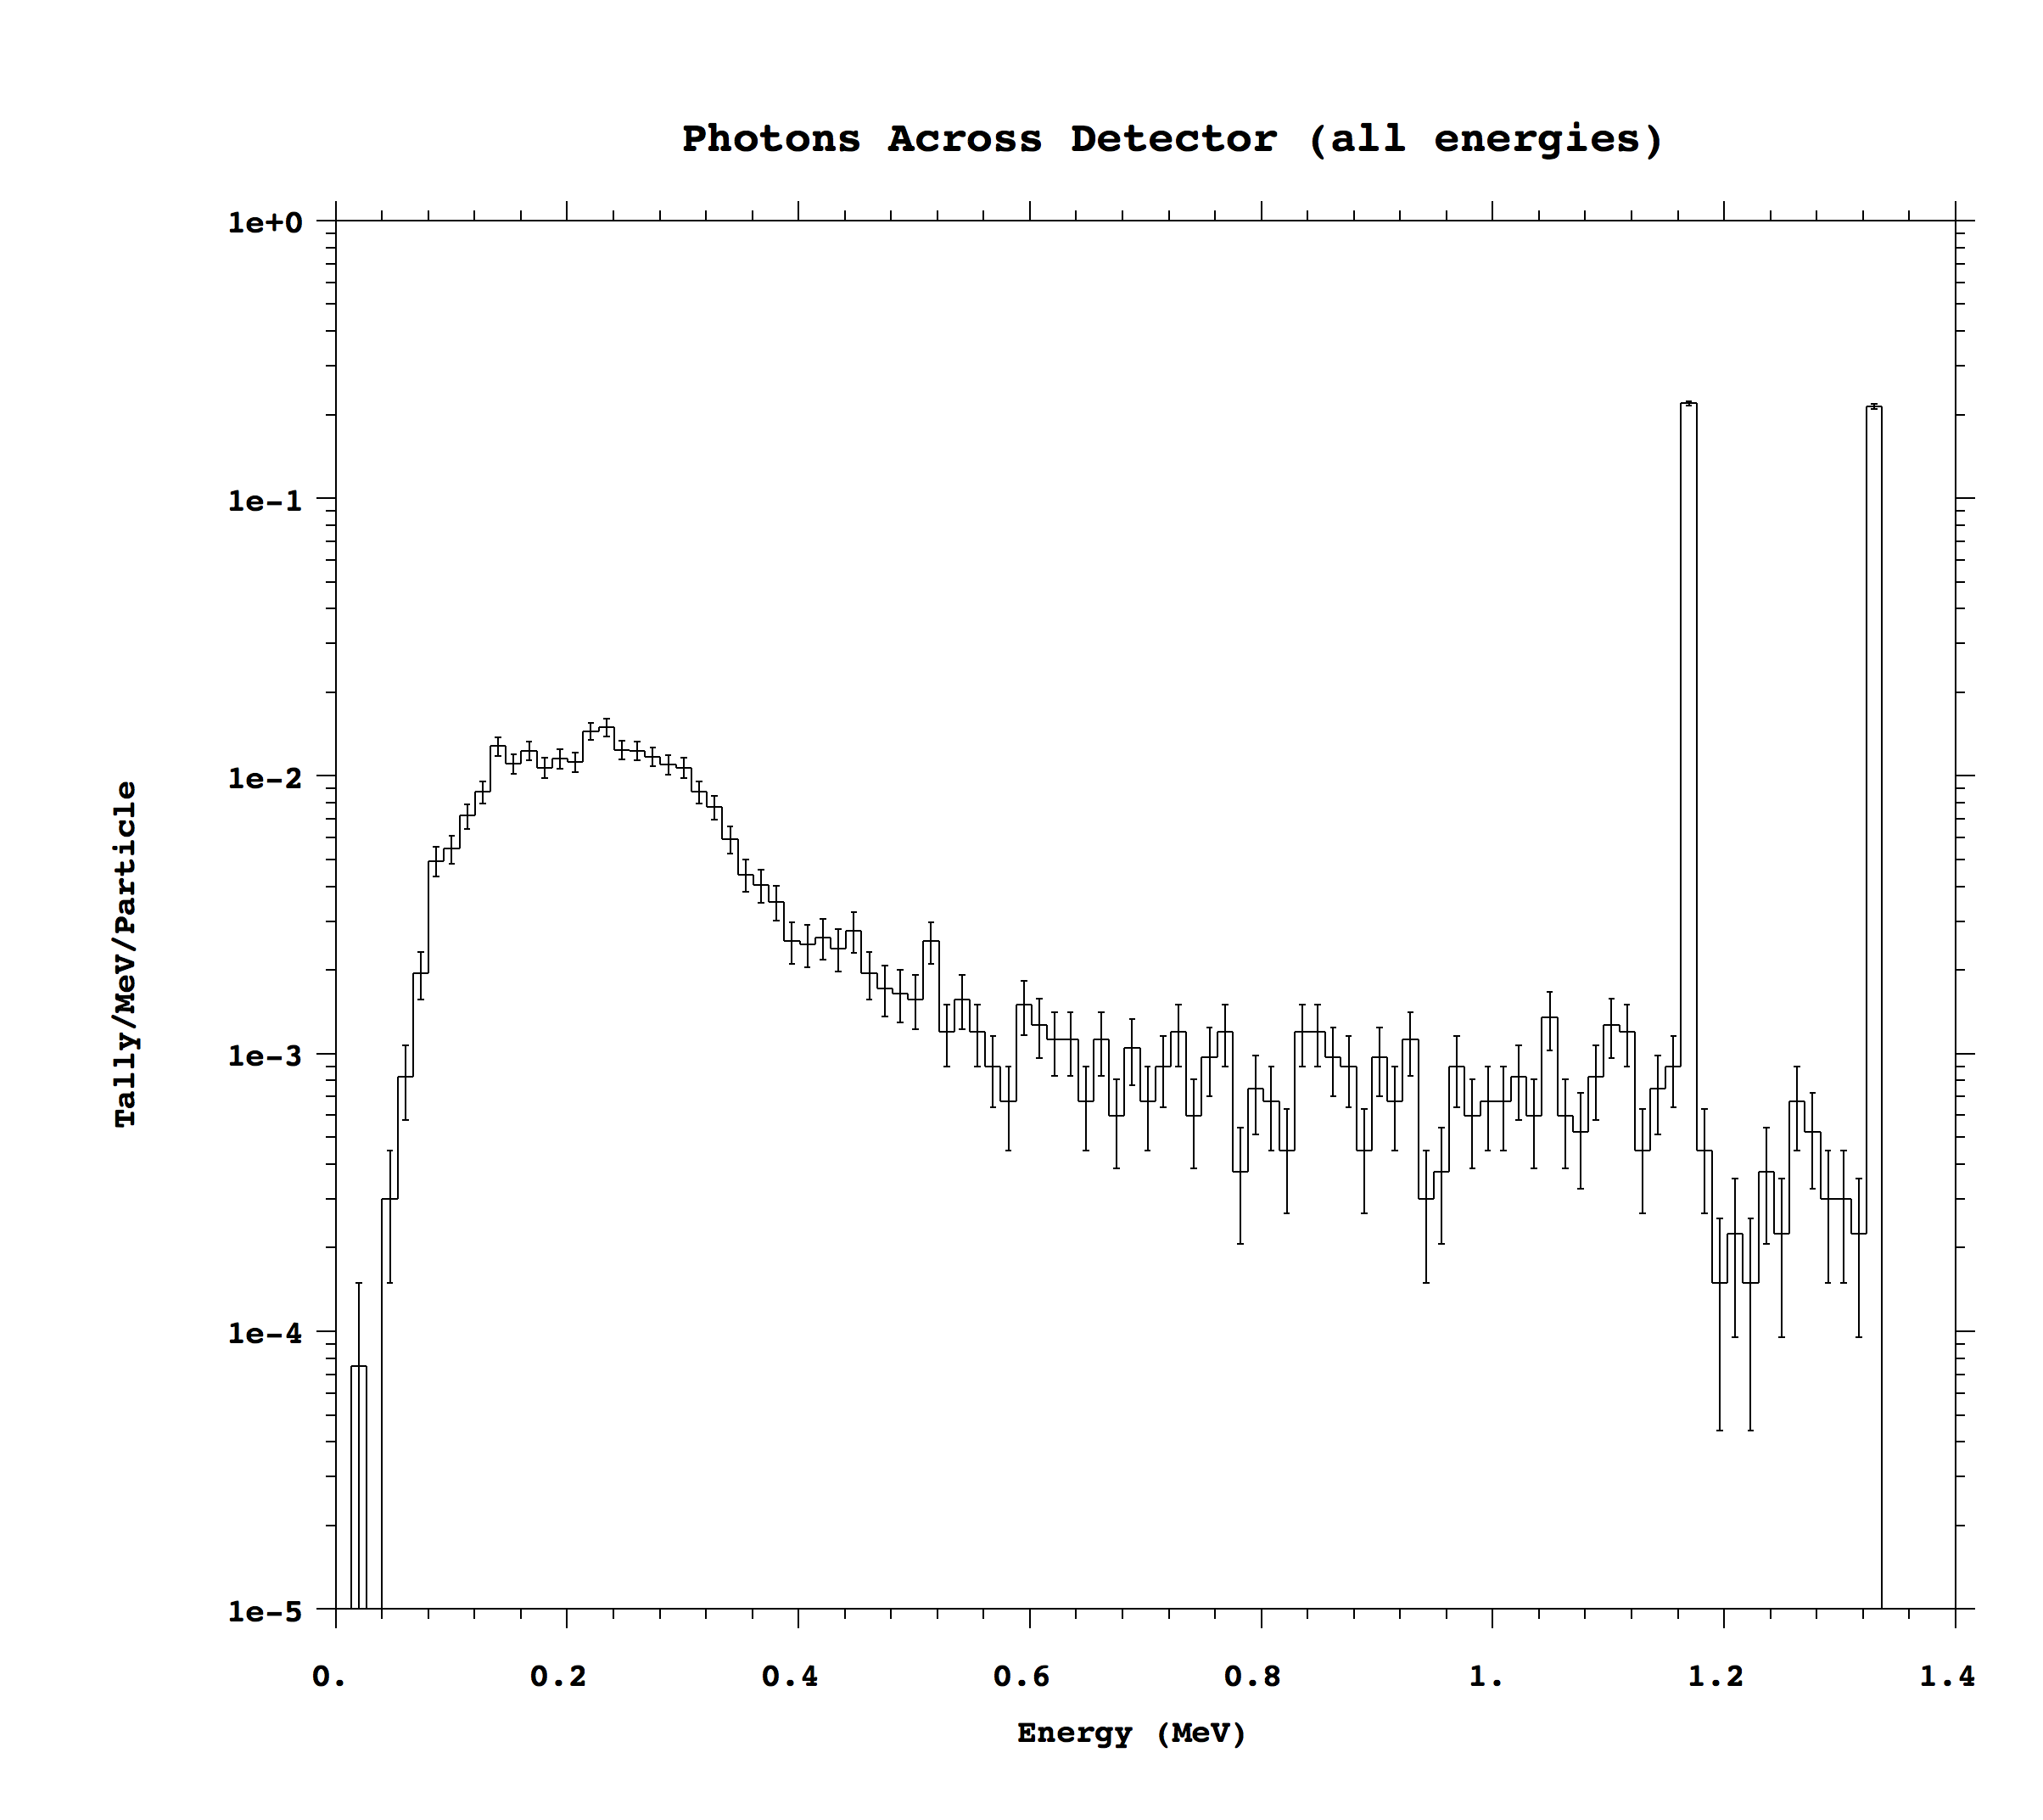
\includegraphics[width=\textwidth]{PhotonEnergyDist}
	\caption[Photons Incident upon Detector]{Photons incident upon a detector from an \iso[60]{Co} source.  The two \iso[60]{Co} photons (\SI{1.17}{\MeV} and \SI{1.33}{\MeV}) make up the majority of the incident photons.}
  \label{fig:PhotonFluxAllEnergies}
\end{figure}
Table \ref{tab:GammaSolidAngle} considers the contributions from all sides, but it is evident that the contributions from the side scattering is not large as 100 times increase in the thickness (\SI{50}{\um} to \SI{5}{\mm}) results in only a 4\% increase in the number of particles crossing the detector.

